\documentclass[aps,pra,reprint,superscriptaddress,nofootinbib,floatfix]{revtex4-2}

\usepackage{amsmath,amssymb,bm}
\usepackage{graphicx}
\usepackage{microtype}
\usepackage{xcolor}
\usepackage[colorlinks=true,linkcolor=blue,citecolor=blue,urlcolor=blue]{hyperref}
\hypersetup{
  pdftitle={Making a simulation framework falsifiable},
  pdfauthor={Ginanjar Utama and Hermawan Kresno Dipojono},
  pdfsubject={Software architecture, evidence labelling, and preregistered
    benchmark gates for operator-centric quantum simulation}
}

\newcommand{\ket}[1]{\lvert #1\rangle}
\newcommand{\avg}[1]{\langle #1\rangle}
\newcommand{\mHa}{\mathrm{mHa}}
\newcommand{\pkg}{\texttt{clifford\_qc}}
\newcommand{\Ctime}{C_{\mathrm{time}}(\epsilon)}
\renewcommand{\labelitemi}{\(\bullet\)}

% Float placement.  Ten of this paper's thirteen floats span both columns, and
% REVTeX can only set those at the top of a page, so the stock settings leave
% white chasms in the text and drift tables pages away from the sentences that
% read them.  Three adjustments, each fixing one of those:
%
% 1. Under the class default (\flushbottom) the text left on a float-heavy page
%    is stretched to fill the column, opening gaps between paragraphs rather
%    than leaving the slack at the foot of the page.
\raggedbottom
%
% 2. A page given over to floats is set with infinitely stretchable glue above,
%    between and below them, which shares the leftover space out as gaps
%    between the floats.  Pin that glue to the foot instead.
\makeatletter
\setlength{\@fptop}{0pt}
\setlength{\@fpsep}{14pt plus 0fil}
\setlength{\@fpbot}{0pt plus 1fil}
\setlength{\@dblfptop}{0pt}
\setlength{\@dblfpsep}{14pt plus 0fil}
\setlength{\@dblfpbot}{0pt plus 1fil}
\makeatother
%
% 3. Keep a page's top from being given over to floats entirely, and make a
%    float-only page earn itself by being almost full: otherwise two wide
%    floats claim a page between them and the reader gets a half-empty spread
%    with the discussion overleaf.
\renewcommand{\dbltopfraction}{0.68}
\renewcommand{\topfraction}{0.8}
\renewcommand{\textfraction}{0.1}
\renewcommand{\dblfloatpagefraction}{0.99}
\renewcommand{\floatpagefraction}{0.85}

% Every quantity quoted in the body text is generated from a committed record
% or from a live census of the source tree; see Sec. VIII.
% source-git-blob-sha: cdcc255e68f6089556c072861baf2aac9b164af9
% source-git-blob-sha: 27a1f47312eeba2b773c1d27ae55f135d5ec2d3e
% source-git-blob-sha: facd47381cebe998bb2b88f9ad1209f1bb162d87
% source-git-blob-sha: 697ff8d08ea51f3a5dd19952b01553bfe8a7cce6
% source-git-blob-sha: 5466fda9e083c2d55b388446e03670b7026f5eec
% source-git-blob-sha: 196bfc37270c18d1376c437b1598e2df918cdda1
% source-git-blob-sha: 5f2faba83d1533d5a8ac4e40432cc294d9aff676
% source-git-blob-sha: 795860f11c1d6baa614683b0035013168a0b0c9b
% source-git-blob-sha: 7e480343cf4271073fa07da75c217d99625ac929
% source-git-blob-sha: 8ff5dcf9f4964092577641033a81423c755b68f6
% generator-git-blob-sha: bf19e8b90c2386577725e510049e8e8951472139
\newcommand{\cqcBankBasis}{\ensuremath{5}}
\newcommand{\cqcBankWords}{\ensuremath{1{,}814}}
\newcommand{\cqcBeHBias}{\ensuremath{0.0033}}
\newcommand{\cqcBeHCXRatio}{\ensuremath{1.15}}
\newcommand{\cqcBeHCXRatioWorst}{\ensuremath{2.79}}
\newcommand{\cqcBeHPrepReduction}{\ensuremath{96.0\%}}
\newcommand{\cqcBeHSettingsFull}{\ensuremath{14}}
\newcommand{\cqcBeHSettingsQWC}{\ensuremath{353}}
\newcommand{\cqcBridgeModules}{\ensuremath{6}}
\newcommand{\cqcCrossAgreeing}{\ensuremath{6}}
\newcommand{\cqcCrossChecked}{\ensuremath{8}}
\newcommand{\cqcDistinctTiers}{\ensuremath{5}}
\newcommand{\cqcFullCertifiedShots}{\ensuremath{2^{24}}}
\newcommand{\cqcGOneExcitation}{\ensuremath{0}}
\newcommand{\cqcGOneMajorana}{\ensuremath{522}}
\newcommand{\cqcGates}{\ensuremath{32}}
\newcommand{\cqcGatesAbsent}{\ensuremath{2}}
\newcommand{\cqcGatesAutomatic}{\ensuremath{20}}
\newcommand{\cqcGatesDispatch}{\ensuremath{10}}
\newcommand{\cqcGatesInWorkflow}{\ensuremath{30}}
\newcommand{\cqcHFourBias}{\ensuremath{3.019}}
\newcommand{\cqcHFourCXAvoided}{\ensuremath{2.22}}
\newcommand{\cqcHFourCXRatio}{\ensuremath{0.45}}
\newcommand{\cqcHFourPrepReduction}{\ensuremath{93.0\%}}
\newcommand{\cqcHFourSettingsFull}{\ensuremath{64}}
\newcommand{\cqcHFourSettingsQWC}{\ensuremath{913}}
\newcommand{\cqcIonRuntimeRatio}{\ensuremath{0.699}}
\newcommand{\cqcJsonRecords}{\ensuremath{28}}
\newcommand{\cqcKStarIon}{\ensuremath{2}}
\newcommand{\cqcKStarIonRegion}{1, 2, 4}
\newcommand{\cqcKStarLogical}{\ensuremath{4}}
\newcommand{\cqcKernelLines}{\ensuremath{2{,}008}}
\newcommand{\cqcLines}{\ensuremath{24{,}894}}
\newcommand{\cqcLogicalRuntimeRatio}{\ensuremath{0.113}}
\newcommand{\cqcMappingSpreadKOne}{\ensuremath{3.48}}
\newcommand{\cqcMeasurementLines}{\ensuremath{3{,}995}}
\newcommand{\cqcModules}{\ensuremath{98}}
\newcommand{\cqcProducers}{\ensuremath{45}}
\newcommand{\cqcProducersWithoutGate}{\ensuremath{25}}
\newcommand{\cqcQWCCertifiedShots}{\ensuremath{2^{29}}}
\newcommand{\cqcRFourAACaseBias}{\ensuremath{0.0695}}
\newcommand{\cqcRFourAACaseWords}{\ensuremath{1{,}223}}
\newcommand{\cqcRFourAAdmissibleBias}{\ensuremath{0.533}}
\newcommand{\cqcRFourACSACaseBias}{\ensuremath{5.90}}
\newcommand{\cqcRFourACSBias}{\ensuremath{5.35}}
\newcommand{\cqcRFourACeiling}{\ensuremath{2{,}048}}
\newcommand{\cqcRFourAFullWords}{\ensuremath{14{,}350}}
\newcommand{\cqcRFourAPassing}{\ensuremath{0}}
\newcommand{\cqcRFourARemovedFraction}{\ensuremath{15.3\%}}
\newcommand{\cqcRFourARungs}{\ensuremath{7}}
\newcommand{\cqcRThreeCCells}{\ensuremath{40}}
\newcommand{\cqcRThreeCCensored}{\ensuremath{2}}
\newcommand{\cqcRThreeCFailures}{\ensuremath{0}}
\newcommand{\cqcRThreeCFinite}{\ensuremath{38}}
\newcommand{\cqcRThreeCSCPriced}{\ensuremath{23}}
\newcommand{\cqcRThreeCSolves}{\ensuremath{19{,}300}}
\newcommand{\cqcRThreeDCells}{\ensuremath{7}}
\newcommand{\cqcRThreeDInstanceSupport}{\ensuremath{4.00}}
\newcommand{\cqcRThreeDMappingSupport}{\ensuremath{2.19}}
\newcommand{\cqcRecordsLabelled}{\ensuremath{14}}
\newcommand{\cqcRecordsNested}{\ensuremath{4}}
\newcommand{\cqcRecordsPerQuantity}{\ensuremath{3}}
\newcommand{\cqcRecordsRoleOnly}{\ensuremath{0}}
\newcommand{\cqcRecordsRoleWithNested}{\ensuremath{2}}
\newcommand{\cqcRecordsUnlabelled}{\ensuremath{5}}
\newcommand{\cqcRitzSupport}{\ensuremath{966}}
\newcommand{\cqcSCFidelityFloor}{\ensuremath{0.50}}
\newcommand{\cqcSCInadmissibleSettings}{\ensuremath{12}}
\newcommand{\cqcSCMeanFidelity}{\ensuremath{0.452}}
\newcommand{\cqcSCSettings}{\ensuremath{14}}
\newcommand{\cqcSameStemPairs}{\ensuremath{20}}
\newcommand{\cqcSeriesFiles}{\ensuremath{21}}
\newcommand{\cqcShotRatio}{\ensuremath{0.03125}}
\newcommand{\cqcShotRatioInverse}{\ensuremath{32}}
\newcommand{\cqcStructuralInstance}{\ensuremath{3.98}}
\newcommand{\cqcStructuralMapping}{\ensuremath{13.07}}
\newcommand{\cqcStructuralMargin}{\ensuremath{0.305}}
\newcommand{\cqcSubspaceLines}{\ensuremath{10{,}101}}
\newcommand{\cqcTargetMilliHartree}{\ensuremath{1.6}}
\newcommand{\cqcTestLines}{\ensuremath{25{,}561}}
\newcommand{\cqcTestModules}{\ensuremath{111}}


\begin{document}

\title{Making a simulation framework falsifiable: one Pauli-word\\
algebra, labelled evidence, and preregistered gates}

\author{Ginanjar Utama}
\email{ginanjar.utama@gmail.com}
\affiliation{Department of Engineering Physics, Institut Teknologi Bandung,
Bandung, Indonesia}

\author{Hermawan Kresno Dipojono}
\email{dipojono@itb.ac.id}
\affiliation{Department of Engineering Physics, Institut Teknologi Bandung,
Bandung, Indonesia}

\date{September 12, 2026}

\begin{abstract}
Quantum simulation software is normally presented through what it can compute.
We present \pkg{} through what it is built to refuse.  Two architectural
commitments carry the design.  First, one sparse Pauli-word algebra underlies
the numerical \texttt{MV} type and the public \texttt{PauliSum}/program
intermediate representation; conversion changes the container exactly, not
the algebraic basis.  The package is \cqcModules{} modules and
\cqcLines{} physical lines against \cqcTestLines{} lines of tests.  Second,
typed numerical paths carry the kind of evidence they produce from the
measurement layer through the solvers, and newer committed records preserve
that label for benchmark gates.  We report what the second commitment
produced.  A dyadic
block-commuting hierarchy reduces a BeH$_2$ bank from \cqcBeHSettingsQWC{} to
\cqcBeHSettingsFull{} compiled settings and certifies the same Ritz functional
at \cqcShotRatio{} of the qubit-wise-commuting shot budget, while a
sparse-connectivity device card refuses \cqcSCInadmissibleSettings{} of those
\cqcSCSettings{} settings outright and prices nothing.  On the one priced
instance, the accuracy-matched block size varies with the card and estimator;
an H$_4$ bank is never priced at all because its own subspace
bias of \cqcHFourBias{}~mHa exceeds the \cqcTargetMilliHartree{}~mHa target.
Two preregistered screens returned no result: mapping spread is not smaller
than instance spread structurally and stays indeterminate after refinement, and
a contextual-restriction screen admitted none of its \cqcRFourARungs{} rungs and
stopped before drawing a sample.  We also report where the contract is not yet
enforced: only \cqcRecordsLabelled{} of \cqcJsonRecords{} committed JSON records
carry a single top-level evidence tier.  None of this is a hardware result, a
scaling result, or an advantage claim.  The contribution is an architecture in
which such claims can fail visibly, together with the record of them failing.
\end{abstract}

\maketitle

\section{Introduction}
\label{sec:introduction}

A research framework for quantum simulation is a claim-generating machine.  It
turns a Hamiltonian into numbers, and those numbers into figures, and the
figures into statements about methods.  Papers describing such frameworks
almost always report the first half of that pipeline: the representation, the
algorithms, the interfaces, the benchmark results that came out well.  The
second half --- what stops a number from being reported as something it is not
--- is usually left to the reader's trust in the authors.

That trust is expensive in this field specifically.  Quantum subspace methods
are compared by basis dimension and energy error, while their dominant
experimental cost sits in state preparations, measurement settings and shot
allocation \cite{mcclean2017qse,huggins2020nonorthogonal,stair2020krylov}.
Finite-shot perturbation of a near-singular overlap matrix is amplified in ways
that a converged exact-simulation table does not show
\cite{epperly2022theory,lee2024sampling,zhang2024measurement}.  An
oracle-evaluated expectation value and a sampled one have the same units and
the same number of digits.  Nothing in a JSON file distinguishes them unless
the architecture makes the distinction and carries it.

This paper describes \pkg{}, an operator-centric framework in the complexified
Clifford algebra $\mathrm{Cl}(2n,\mathbb{C}) \cong M(2^n,\mathbb{C})$, and it
takes the second half of the pipeline as its subject.  The representation and
the solvers are described in companion manuscripts
\cite{utama2026operatorcentric}; here they are the setting, not the claim.  The
claim is that two architectural commitments --- one algebra shared across an
explicit intermediate-representation boundary, and evidence labels carried by
the typed numerical paths --- make a
particular class of over-claim structurally difficult, and that the resulting
evidence record is unusually full of results that did not work.

We defend that claim in three steps.

\begin{enumerate}
  \item \textbf{The architecture, measured rather than described}
  (Sec.~\ref{sec:architecture}).  Every module of the package is assigned to
  exactly one layer, and the assignment is checked against the source tree when
  this manuscript is built, so Table~\ref{tab:layers} cannot drift from the code
  it describes.  Import-time dependencies point downward only; the upward edges
  that exist are deferred to call time and are named individually.

  \item \textbf{The evidence contract} (Secs.~\ref{sec:evidence} and
  \ref{sec:gates}).  An evidence vocabulary threads from the measurement layer
  into the committed records, and the benchmark layer is a pairing of record
  producers with gates that assert different things.  We report the coverage of
  both honestly, including where the contract is a convention rather than an
  enforced invariant.

  \item \textbf{What the contract admitted, and what it stopped}
  (Secs.~\ref{sec:admitted} and \ref{sec:stopped}).  The positive results are
  measurement-structural and cost-structural, and each is stated with the axis
  it does not generalize along.  The negative and indeterminate results are
  given the same space as the positive ones, because in this architecture they
  are the same kind of object: a preregistered question, a declared gate, and
  the outcome the gate returned.
\end{enumerate}

What this paper is not: it is not a performance comparison against Qiskit,
PennyLane, \textsc{pytket}, OpenFermion or PyZX, which \pkg{} reaches through
\cqcBridgeModules{} optional bridge modules rather than competing with
\cite{mcclean2020openfermion}; it is not a hardware study; and it contains no advantage claim of any kind.  Every device cost in
this paper is a logical accounting under an explicitly illustrative device
card, and every card in the records carries a field saying so.

\section{One algebra, and the seams around it}
\label{sec:architecture}

\subsection{The end-to-end contract}

\begin{figure*}
  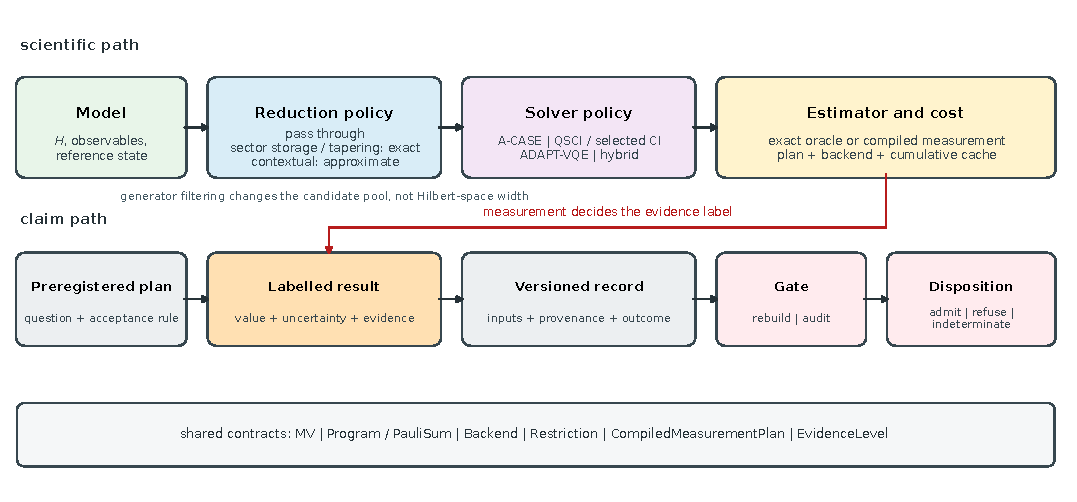
\includegraphics[width=\textwidth]{paper_assets/architecture_flow.pdf}
  \caption{The end-to-end architecture, separating a scientific result from a
  publishable claim.  The scientific path constructs a model, applies only
  explicit reductions, selects a solver policy, and evaluates an exact or
  measured estimator.  The claim path attaches evidence, writes provenance,
  and lets a declared gate admit, refuse, or leave the result indeterminate.
  The band at the foot names the typed contracts shared across both paths.
  Generator filtering changes the candidate pool; it is not shown as a
  Hilbert-space reduction.}
  \label{fig:architecture-flow}
\end{figure*}

Figure~\ref{fig:architecture-flow} makes explicit a distinction that a layer
inventory alone cannot show.  Sector representation compresses exact storage;
symmetry tapering reduces the active register exactly; contextual restriction
reduces it approximately and carries the removed Hamiltonian fraction as a
bias source; and A-CASE or determinant projection reduces only the subsequent
generalized eigenproblem.  Generator filtering changes which directions may
enter that projected solve, not the Hilbert space itself.  Those operations
therefore remain separate policies even though they meet at one restriction
and solver interface.

\subsection{The kernel}

The numerical kernel's canonical operator type is the multivector \texttt{MV}, a
sparse map from packed Pauli-word codes to complex coefficients, two bits per
qubit, with multiplication implemented as exclusive-or, and-mask and
population count modulo four.  States, gates, Kraus channels, Jordan--Wigner
Clifford generators and fermionic creation and annihilation operators lower to
this type.  The public program intermediate representation also exposes a
distinct immutable \texttt{PauliSum} container for Hamiltonians and
observables.  Its \texttt{to\_mv} and \texttt{from\_mv} boundary is exact and
uses the same packed word codes; it is a real container conversion, but not a
change of algebraic basis or operator semantics.  Benchmarks therefore need
not own a basis-translation convention, while the architecture still names
the boundary that the public API actually has.

Three distinct pairings are defined on \texttt{MV} and are deliberately not
interchangeable; the reference-state pairing used to reconstruct projected
matrix elements is not the Hilbert--Schmidt pairing used to measure how much of
a Hamiltonian a restriction removed.  Keeping them separate is what lets
Sec.~\ref{sec:stopped} report a removed Hamiltonian fraction as a bias source
rather than as a resource saving.

\subsection{Layers as a partition, not a picture}

\begin{figure*}
  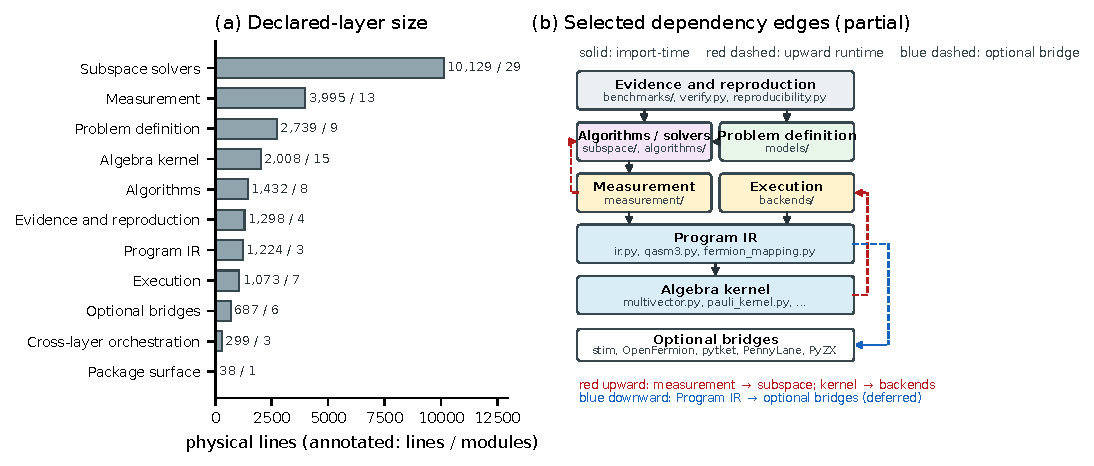
\includegraphics[width=\textwidth]{paper_assets/layer_stack.pdf}
  \caption{The package as measured.  (a) Physical lines per declared layer,
  annotated with lines and module count; the census is recomputed from the
  source tree whenever this manuscript is rebuilt.  (b) The layer stack.  Solid
  arrows are import-time dependencies, which point downward only: no package
  initialization reaches upward, so importing a lower layer never drags a
  higher one in.  Red dashed arrows are genuine upward runtime edges deferred
  to call time; the blue dashed arrow is a downward call into an optional
  bridge.  The deferral buys initialization order, not independence, and
  Sec.~\ref{sec:architecture} states them individually rather than claiming an
  acyclic runtime graph.}
  \label{fig:layers}
\end{figure*}

\begin{table}
  \caption{Declared layers of \pkg{}, recomputed from the source tree at
  manuscript build time.  The share column is of package lines; the test suite
  is listed for scale and is not a layer.}
  \label{tab:layers}
  \begin{ruledtabular}
  \begin{tabular}{lrrr}
  Layer & Modules & Lines & Share \\
  \colrule
  % source-git-blob-sha: ed6aff674b9327cdefff5dbe38f9a5bcca56cf53
% generator-git-blob-sha: b574dd5585871ad9ade1e0da4d5be70359947048
Algebra kernel & \ensuremath{15} & \ensuremath{2{,}003} & \ensuremath{8.6\%} \\
Program IR & \ensuremath{3} & \ensuremath{1{,}209} & \ensuremath{5.2\%} \\
Execution & \ensuremath{7} & \ensuremath{1{,}058} & \ensuremath{4.6\%} \\
Measurement & \ensuremath{13} & \ensuremath{3{,}924} & \ensuremath{16.9\%} \\
Problem definition & \ensuremath{8} & \ensuremath{2{,}338} & \ensuremath{10.1\%} \\
Algorithms & \ensuremath{8} & \ensuremath{1{,}428} & \ensuremath{6.1\%} \\
Subspace solvers & \ensuremath{28} & \ensuremath{9{,}579} & \ensuremath{41.2\%} \\
Cross-layer orchestration & \ensuremath{1} & \ensuremath{31} & \ensuremath{0.1\%} \\
Evidence and reproduction & \ensuremath{3} & \ensuremath{966} & \ensuremath{4.2\%} \\
Optional bridges & \ensuremath{6} & \ensuremath{667} & \ensuremath{2.9\%} \\
Package surface & \ensuremath{1} & \ensuremath{38} & \ensuremath{0.2\%} \\
\colrule
Package total & \ensuremath{93} & \ensuremath{23{,}241} & \ensuremath{100.0\%} \\
Test suite & \ensuremath{104} & \ensuremath{23{,}530} & --- \\

  \end{tabular}
  \end{ruledtabular}
\end{table}

Figure~\ref{fig:layers} and Table~\ref{tab:layers} report the package as it is
on the branch that produced this manuscript: \cqcModules{} modules and
\cqcLines{} physical lines, against a test suite of \cqcTestModules{} modules
and \cqcTestLines{} lines.  The distribution is lopsided on purpose.  The
algebra kernel is \cqcKernelLines{} lines; the subspace solvers are
\cqcSubspaceLines{}, and the measurement layer is \cqcMeasurementLines{}.  A
framework whose kernel is under a tenth of its body is one where the
interesting work is in the layers that decide what a measurement costs and what
a number means.  That solver layer carries the operator-response subspace
eigensolver of the companion manuscripts beside sampled-determinant and
adaptive variational arms \cite{peruzzo2014vqe,grimsley2019adapt,kanno2026qsci},
classical selected-configuration-interaction controls, and their hybrids, each
scored against the same oracles.

The layer assignment in Table~\ref{tab:layers} is a declared partition.  The
generator refuses to emit the table unless every module in the package lands in
exactly one layer, so a module added without an architectural decision fails
the build of this manuscript rather than quietly widening a row.

\subsection{The seams}

Replaceability lives in a small number of typed interfaces: the operator
\texttt{MV}; the program intermediate representation, whose Pauli rotors
$\exp(-\mathrm{i}\theta P/2)$ and named Cliffords lower exactly to \texttt{MV};
the backend protocol, which is the only way the algorithm layer reaches
execution; the group-sample contract, which carries either a qubit-wise
commuting setting identified by its per-qubit basis or a Clifford-diagonalized
setting with an explicit key and signed readout map; the frozen model type; the
labelled basis direction; the compiled measurement plan; and the symmetry
restriction.  Changing one of these is a cross-cutting change and changing
anything else is local.  That is the whole architectural content of the layer
diagram, and it is why the group-sample contract in particular is shaped the
way it is: without one type that carries both measurement forms, the
block-commuting results of Sec.~\ref{sec:admitted} could not feed the same
estimators without pretending they were measured qubit-wise.

The upward edges deserve their own sentence, because a paper claiming an
acyclic architecture while shipping function-scope imports upward would be
making exactly the kind of unfalsifiable claim this paper is about.  The
measurement layer imports the subspace layer inside methods; the kernel reaches
into the execution layer from function scope for sector helpers; and the
optional bridges are kept out of every package initializer, either by
function-scope import or by not being re-exported, so that reaching them
requires naming them.  Collapsed to the package level, the call-time graph is
not acyclic.  The invariant the package actually enforces is about when, not
about how many.

\section{Where a number acquires its label}
\label{sec:evidence}

\begin{figure*}
  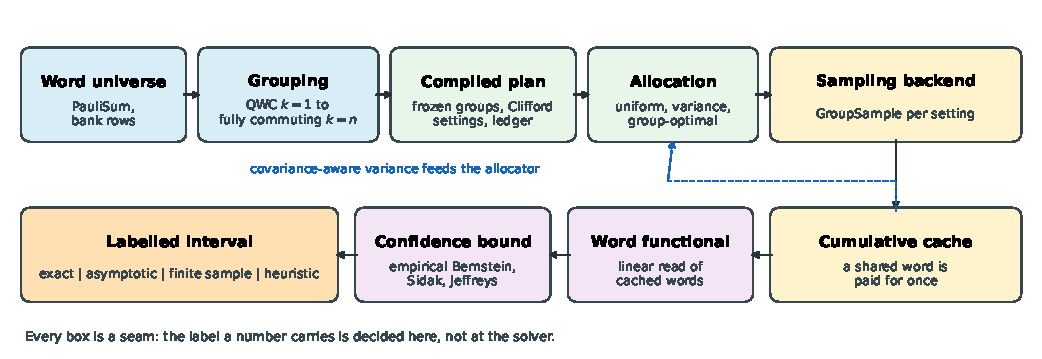
\includegraphics[width=\textwidth]{paper_assets/evidence_path.pdf}
  \caption{One pass from a word universe to a labelled interval.  The label is
  decided in the measurement layer, not at the solver: an oracle-evaluated
  expectation and a sampled one traverse different boxes and arrive carrying
  different evidence, which is what allows the benchmark gates of
  Sec.~\ref{sec:gates} to compare like with like.}
  \label{fig:evidence}
\end{figure*}

The measurement layer is the largest non-solver layer because it is where an
expectation value stops being a float and becomes a claim.
Figure~\ref{fig:evidence} shows one pass.  A word universe is grouped, either
qubit-wise or under dyadic block commutativity; the grouping is frozen into a
compiled plan with signed parity readouts, a matched resource ledger, and
Clifford settings synthesized through a stabilizer tableau
\cite{gidney2021stim,verteletskyi2020grouping,crawford2021efficient,miller2024hardware}; shots
are allocated; the sampling backend returns joint outcome histograms per
setting; a cumulative cache pays for a shared word once across observables; a
linear functional reads the cache; and a confidence bound turns the read into
an interval with a stated family and failure probability.

Typed numerical paths use the small \texttt{EvidenceLevel} vocabulary: exact,
asymptotic, finite-sample, heuristic, or none.  Committed records do not yet
share that closed enum: some use producer-specific scope or composite labels,
including structural and exact-oracle/finite-sample labels, and the census
reports those strings rather than normalizing them.  The purpose of the typed
vocabulary is not taxonomy but prevention.  An
exact-tier subspace bias and a finite-sample statistical radius have the same
units and combine into one accuracy target, but they are not the same evidence,
and a Pareto front computed across both would be meaningless.  In this
architecture the front is computed only inside one evidence category.

\subsection{Where the contract is convention rather than invariant}

\begin{table}
  \caption{How the committed record set declares the evidence its numbers
  carry.  Counts are recomputed from
  \texttt{benchmarks/reference\_results/} at manuscript build time.}
  \label{tab:evidence}
  \scriptsize
  \begin{ruledtabular}
  \begin{tabular}{@{}lrl@{}}
  Declaration form & Records & Example \\
  \colrule
  % source-git-blob-sha: d3f96c8fd93e44753cc1b7ba0577b9820c56785d
% generator-git-blob-sha: b574dd5585871ad9ade1e0da4d5be70359947048
Top-level tier & \ensuremath{14} & \texttt{bank-storage-ledger} \\
Per-quantity mapping & \ensuremath{3} & \texttt{fcidump-h4} \\
Role plus nested tier & \ensuremath{2} & \texttt{qr3b-instance-preflight} \\
Role, not a tier & \ensuremath{0} & --- \\
Tier basis, not a tier & \ensuremath{0} & --- \\
Nested in sub-object & \ensuremath{4} & \texttt{clifford-hierarchy-beh2} \\
No evidence & \ensuremath{5} & \texttt{clifford-hierarchy-beh2-v2} \\
\colrule
JSON records & \ensuremath{28} & \ensuremath{5} tier strings \\
Series files (JSONL, CSV, MD) & \ensuremath{21} & not inspected here \\

  \end{tabular}
  \end{ruledtabular}
\end{table}

Table~\ref{tab:evidence} reports the coverage honestly, and it is the least
flattering table in this paper.  Of \cqcJsonRecords{} committed JSON records,
\cqcRecordsLabelled{} declare a single top-level evidence tier, drawn from
\cqcDistinctTiers{} distinct tier strings; \cqcRecordsPerQuantity{} declare a
per-quantity mapping instead, because their producers report several quantities
at different tiers in one file; \cqcRecordsNested{} nests the tier inside a
sub-object; \cqcRecordsRoleWithNested{} declare an evidence \emph{role} at the
top level and tiers inside sub-objects; \cqcRecordsRoleOnly{} carry a role with
no tier at all; and \cqcRecordsUnlabelled{} carry no record-level
evidence field whatsoever.  A further \cqcSeriesFiles{} non-JSON series files
--- line-delimited JSON, CSV and Markdown summaries --- are counted but not
inspected for per-row declarations by this census.

This is a real gap and it is worth stating precisely.  \texttt{EvidenceLevel}
is enforced in typed numerical paths, where one selection module defines it
and the measurement and subspace layers carry it in their return types.  Newer
records preserve evidence at the top level, but the broader record-label
vocabulary is not normalized and is not enforced by a schema over the
record set: nothing today rejects a new record that omits the field.  The
census that produced Table~\ref{tab:evidence} is recomputed whenever this
manuscript is rebuilt, so the number cannot silently improve or decay, but a
census is a measurement, not a gate.  Closing that gap --- a required tier field
validated for every committed record --- is the single most valuable change we
can identify to the contract described here.

\section{Producers, gates, and preregistration}
\label{sec:gates}

The benchmark directory is not a scratch space; it is a two-part contract, and
the pairing is the architecture.  \cqcProducers{} producers write records.
\cqcGates{} gates read them.  \cqcGatesInWorkflow{} are named in the
continuous-integration workflow, and the distinction inside that number
matters: \cqcGatesAutomatic{} run on every pull request, while
\cqcGatesDispatch{} run only when dispatched by hand, because they draw
replicas and cost runner-hours.  \cqcGatesAbsent{} exist in the repository but
in no workflow at all.  Each gate that does run is its own named step, and each
executes even after an earlier one fails, so that a drift suite reports every
symptom rather than the first.

\begin{table}
  \caption{What each class of benchmark gate asserts.  Counts are recomputed
  from \texttt{benchmarks/} at manuscript build time, and the generator refuses
  to emit the table unless every gate on disk has a declared class.}
  \label{tab:gates}
  \footnotesize
  \begin{ruledtabular}
  \begin{tabular}{lrp{0.42\columnwidth}}
  Class & Gates & Asserts \\
  \colrule
  % source-git-blob-sha: 97f8f2bb1bdb16698ed983fa6b3d62dc27749d43
% generator-git-blob-sha: 045582ef83ef5c9b1d47f8166ebb88a9158d284b
Value-rebuilt & \ensuremath{18} & recomputes its same-stem producer's record and fails on numeric drift \\
Preregistration & \ensuremath{5} & compares a predeclared plan against committed constants; no rebuild \\
Lineage and environment & \ensuremath{3} & provenance stamping, environment migration, regeneration identity \\
Plan ledger & \ensuremath{1} & the phase status file against the plan document and the source tree \\
Documentation & \ensuremath{1} & every documented command, flag, constant, and record still exists \\
Cross-artifact & \ensuremath{2} & a record against an artifact produced outside benchmarks/ \\
\colrule
Gates, all classes & \ensuremath{30} & \ensuremath{28} named in the CI workflow \\
Run on every pull request & \ensuremath{18} & \ensuremath{10} more by manual dispatch \\
Producers & \ensuremath{42} & \ensuremath{18} have a same-stem gate \\
Producers with no value gate & \ensuremath{24} & manuscript evidence, drivers, exploratory output \\

  \end{tabular}
  \end{ruledtabular}
\end{table}

The temptation in a paper like this one is to write that every record is
re-derived.  It is not, and Table~\ref{tab:gates} says so.  Only
\cqcSameStemPairs{} producers have a same-stem gate that recomputes their record
and fails on numeric drift.  The other \cqcProducersWithoutGate{} write
manuscript evidence, paper-suite drivers, or exploratory output with no value
gate.  The most important of those is stated in the reproduction documentation
rather than excused: the validation-ladder record is manuscript evidence for a
companion paper, and regenerating it would move published inputs across all its
families, so no gate rebuilds it.

The remaining gate classes matter for how the negative results of
Sec.~\ref{sec:stopped} should be read.  Five gates are preregistration gates:
they compare a plan declared before any sampling against the constants
committed with the result, and they rebuild nothing.  This is the mechanism
that makes a null result reportable.  A screen whose acceptance rule, accuracy
target, margin factor, word-universe ceiling and block sizes were all committed
in a configuration file, with a merge commit and a content hash, before any
sample was drawn, can return ``no rung admitted'' without that outcome being a
choice made after seeing the data \cite{nosek2018preregistration}.  Three
further gates check lineage and environment rather than values, one checks the
plan ledger against the source tree, one checks that the reproduction
documentation still describes the code it claims to reproduce, and two compare
records against artifacts produced outside the benchmark directory.

Two properties of the execution environment are load-bearing and are worth
recording because they bound what reproduction means here.  Continuous
integration pins one thread for the numerical libraries, because threaded
basic-linear-algebra reductions sum in a thread-count-dependent order and the
same symmetric eigensolve returns different last bits across thread counts.
That closes the one source of nondeterminism a workflow can close.  It does not
make records portable across processor microarchitectures, because kernel
selection by instruction set remains, and the reproduction documentation records
that floor rather than claiming bit-exact portability
\cite{peng2011reproducible,wilson2017practices}.

\section{What the architecture admitted}
\label{sec:admitted}

This section reports the positive results the contract let through.  Each is
structural or cost-structural, each is on small instances, and each is stated
with the axis along which it does not generalize.

\subsection{The block-commuting hierarchy is a real trade, and it is
instance-dependent}

Commuting-group measurement is usually presented as a setting-count reduction.
Under the dyadic hierarchy --- two words are compatible when their restrictions
commute inside every contiguous $k$-qubit block, so $k=1$ is exactly qubit-wise
commutation and $k=n$ is full commutation --- the reduction is real and large.
On the H$_4$ bank, compiled settings fall from \cqcHFourSettingsQWC{} to
\cqcHFourSettingsFull{}, a preparation reduction of \cqcHFourPrepReduction{}.
On the BeH$_2$ bank they fall from \cqcBeHSettingsQWC{} to
\cqcBeHSettingsFull{}, a reduction of \cqcBeHPrepReduction{}.

\begin{table*}
  \caption{The dyadic block-commuting hierarchy on two committed banks.  The
  last column is the added logical entangling cost divided by the avoided
  preparation cost, both measured against the $k=1$ rung of the same bank; it
  is undefined at $k=1$.  All-to-all logical Clifford circuits, no routing,
  noise or mitigation.}
  \label{tab:hierarchy}
  \begin{ruledtabular}
  \begin{tabular}{llrrrrr}
  Bank & $k$ & Settings & Mean CX per setting & Max CX depth & Preparations at uniform shots & CX cost over avoided preparation \\
  \colrule
  % source-git-blob-sha: 27a1f47312eeba2b773c1d27ae55f135d5ec2d3e
% source-git-blob-sha: facd47381cebe998bb2b88f9ad1209f1bb162d87
% generator-git-blob-sha: b574dd5585871ad9ade1e0da4d5be70359947048
H$_4$ & \ensuremath{1} & \ensuremath{913} & \ensuremath{0.0} & \ensuremath{0} & \ensuremath{7{,}304{,}000} & --- \\
 & \ensuremath{2} & \ensuremath{647} & \ensuremath{4.3} & \ensuremath{4} & \ensuremath{5{,}176{,}000} & \ensuremath{0.09} \\
 & \ensuremath{4} & \ensuremath{238} & \ensuremath{13.8} & \ensuremath{14} & \ensuremath{1{,}904{,}000} & \ensuremath{0.21} \\
 & \ensuremath{8} & \ensuremath{64} & \ensuremath{29.5} & \ensuremath{35} & \ensuremath{512{,}000} & \ensuremath{0.45} \\
\colrule
BeH$_2$ & \ensuremath{1} & \ensuremath{353} & \ensuremath{0.0} & \ensuremath{0} & \ensuremath{2{,}824{,}000} & --- \\
 & \ensuremath{2} & \ensuremath{41} & \ensuremath{2.7} & \ensuremath{1} & \ensuremath{328{,}000} & \ensuremath{2.79} \\
 & \ensuremath{4} & \ensuremath{26} & \ensuremath{7.4} & \ensuremath{10} & \ensuremath{208{,}000} & \ensuremath{1.69} \\
 & \ensuremath{8} & \ensuremath{14} & \ensuremath{21.1} & \ensuremath{23} & \ensuremath{112{,}000} & \ensuremath{1.15} \\

  \end{tabular}
  \end{ruledtabular}
\end{table*}

\begin{figure*}
  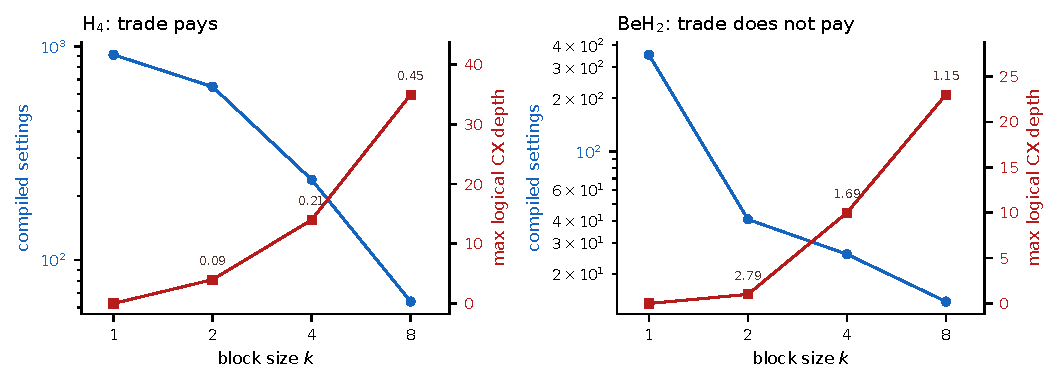
\includegraphics[width=\textwidth]{paper_assets/hierarchy_tradeoff.pdf}
  \caption{Compiled settings (left axis, blue) and maximum logical entangling
  depth per setting (right axis, red) along the block-size axis, for the two
  committed banks.  Annotations give the added entangling cost over the avoided
  preparation cost against $k=1$; the verdict in each title is that ratio
  against unity.  The protocol is identical on both panels, and the trade
  changes sign between them.}
  \label{fig:hierarchy}
\end{figure*}

What the ledger adds is the other half of the trade, and it does not point the
same way on both instances.  Table~\ref{tab:hierarchy} and
Fig.~\ref{fig:hierarchy} report, at each rung, the added logical entangling
cost against the avoided preparation cost.  On H$_4$ that ratio stays below one
at every rung, reaching \cqcHFourCXRatio{} at full commutation: the trade pays
under an all-to-all logical model, at \cqcHFourCXAvoided{} logical entangling
applications per avoided preparation.  On BeH$_2$ the ratio exceeds one at every
rung above qubit-wise, reaching \cqcBeHCXRatioWorst{} at $k=2$ and falling only
to \cqcBeHCXRatio{} at full commutation: the same protocol on a different bank
costs more entangling depth than it saves in preparations.  A framework that
reported settings alone would have reported these two instances as the same
result.

\subsection{A certified shot reduction, and a card that refuses it}

\begin{table*}
  \caption{Qubit-wise against fully commuting measurement on one frozen
  BeH$_2$ bank, from the preregistered comparison.  The ratio column is the
  fully commuting value over the qubit-wise value.  Runtimes are
  accuracy-matched logical accounting under illustrative device cards, not
  hardware measurements.}
  \label{tab:phase14b}
  \begin{ruledtabular}
  \begin{tabular}{lrrr}
  Quantity & QWC ($k=1$) & Full ($k=8$) & Ratio \\
  \colrule
  % source-git-blob-sha: 697ff8d08ea51f3a5dd19952b01553bfe8a7cce6
% generator-git-blob-sha: 8e04e5c6a087442543c3cd5c63de73fade834c8d
Compiled settings & \ensuremath{353} & \ensuremath{14} & \ensuremath{0.040} \\
Settings the Ritz functional touches & \ensuremath{179} & \ensuremath{7} & \ensuremath{0.039} \\
Readable word--setting pairs & \ensuremath{4{,}790} & \ensuremath{3{,}284} & \ensuremath{0.686} \\
One-qubit gates, summed over settings & \ensuremath{3{,}648} & \ensuremath{297} & \ensuremath{0.081} \\
Two-qubit gates, summed over settings & \ensuremath{0} & \ensuremath{296} & --- \\
Certified total physical shots & \ensuremath{2^{29}} & \ensuremath{2^{24}} & \ensuremath{0.03125} \\
\colrule
$C_{\mathrm{time}}(\epsilon)$, ion-like (s) & \ensuremath{134{,}835} & \ensuremath{94{,}291} & \ensuremath{0.699} \\
$C_{\mathrm{time}}(\epsilon)$, logical-alltoall (s) & \ensuremath{1{,}108} & \ensuremath{125} & \ensuremath{0.113} \\
$C_{\mathrm{time}}(\epsilon)$, superconducting-like (s) & \ensuremath{2{,}294} & inadmissible & --- \\
Settings below the fidelity floor, superconducting-like & \ensuremath{0} & \ensuremath{12} & --- \\

  \end{tabular}
  \end{ruledtabular}
\end{table*}

The setting count is not the estimand.  The preregistered comparison of
Table~\ref{tab:phase14b} fixes one BeH$_2$ bank of \cqcBankWords{} measured
words supporting a \cqcBankBasis{}-vector subspace, and asks for the total
physical shots at which the first-order Ritz energy functional is certified
inside a stochastic radius, under a two-sided empirical Bernstein bound with a
declared family and failure probability
\cite{maurer2009empirical,sidak1967rectangular}, with the same allocation rule
on both arms.

The fully commuting arm is certified at \cqcFullCertifiedShots{} total physical
shots against \cqcQWCCertifiedShots{} for the qubit-wise arm: a ratio of
\cqcShotRatio{}, or one part in \cqcShotRatioInverse{}.  That is a larger effect
than the setting-count reduction alone would suggest, because the Ritz
functional touches only part of the bank --- its measured support is
\cqcRitzSupport{} of the \cqcBankWords{} assigned words, concentrated on
\cqcSCSettings{} compiled settings rather than spread over
\cqcBeHSettingsQWC{} --- and concentration is what lets the allocator buy the
variance down with fewer shots.

Then the device cards are applied, and the result splits.  On the all-to-all
logical baseline the fully commuting arm costs \cqcLogicalRuntimeRatio{} of the
qubit-wise runtime.  On the slow-gate all-to-all card it costs
\cqcIonRuntimeRatio{}: still cheaper, but most of the shot saving is consumed by
two-qubit gate time, since that arm's settings carry entangling gates and the
qubit-wise arm's carry none.  On the sparse-connectivity card the comparison
does not happen at all.  \cqcSCInadmissibleSettings{} of the fully commuting
arm's \cqcSCSettings{} compiled settings fall below the card's fidelity floor
once the routing surrogate is applied --- mean setting fidelity
\cqcSCMeanFidelity{} against a floor of \cqcSCFidelityFloor{} --- so the ledger
returns \emph{inadmissible} rather than a number.

We draw attention to that last cell rather than burying it.  An architecture
that priced everything would have reported a runtime for that card, and it
would have been a runtime for a protocol the card cannot execute at the stated
fidelity.  Refusing to price is the correct output, and it is only available
because admissibility is part of the cost type rather than a caveat in prose.

\subsection{The accuracy-matched block size depends on the card and estimator}

The deeper cost question is not which protocol uses fewer settings but which
one reaches a stated accuracy for the least device time.  Writing $\Ctime$ for
the accuracy-matched logical runtime at target $\epsilon$, the search prices
each (mapping, block size) cell by bracketing the shot budget at which the
replica root-mean-square error of the selected-rank Ritz energy clears the
target, with a zero-failure gate and a one-sided bootstrap bound
\cite{efron1979bootstrap}.

\begin{table*}
  \caption{Accuracy-matched cost of the priced BeH$_2$ instance on the
  Jordan--Wigner arm, at the \cqcTargetMilliHartree{}~mHa target.  $k^*$ is the
  set of rungs whose cost interval reaches the smallest upper bound; the status
  column is the record's own resolution state.  The spread column is over all
  five mapping arms at the same rung.}
  \label{tab:cost}
  \footnotesize
  \begin{ruledtabular}
  \begin{tabular}{llrllrlr}
  Device card & Estimator & $k^*$ point & $k^*$ region & Status & $\Ctime$ at $k^*$ (s) & Cheapest mapping & Mapping spread \\
  \colrule
  % source-git-blob-sha: 5466fda9e083c2d55b388446e03670b7026f5eec
% generator-git-blob-sha: d4dfc704534ba3e9ea7f5cff4c04b8793b7bfde0
ion-like & single assignment & \ensuremath{2} & 1, 2, 4 & region & \ensuremath{364} & \texttt{bk+2q} & \ensuremath{1.74} \\
ion-like & pooled & \ensuremath{2} & 1, 2 & region & \ensuremath{91.1} & \texttt{bk+2q} & \ensuremath{1.74} \\
logical-alltoall & single assignment & \ensuremath{4} & 1, 2, 4, 8 & region & \ensuremath{1.55} & \texttt{bk} & \ensuremath{3.87} \\
logical-alltoall & pooled & \ensuremath{2} & 1, 2, 4, 8 & region & \ensuremath{0.425} & \texttt{bk+2q} & \ensuremath{1.62} \\
superconducting-like & single assignment & \ensuremath{2} & 1, 2, 4 & region & \ensuremath{4.33} & \texttt{bk+2q} & \ensuremath{1.84} \\
superconducting-like & pooled & \ensuremath{2} & 1, 2 & region & \ensuremath{1.08} & \texttt{bk+2q} & \ensuremath{1.84} \\
\colrule
\multicolumn{8}{p{0.96\textwidth}}{Rungs the superconducting-like card refuses to price: $k={8}$. Accuracy target \ensuremath{1.6} mHa; H$_4$ is not priced at all, its own subspace bias being \ensuremath{3.019} mHa.} \\

  \end{tabular}
  \end{ruledtabular}
\end{table*}

\begin{figure*}
  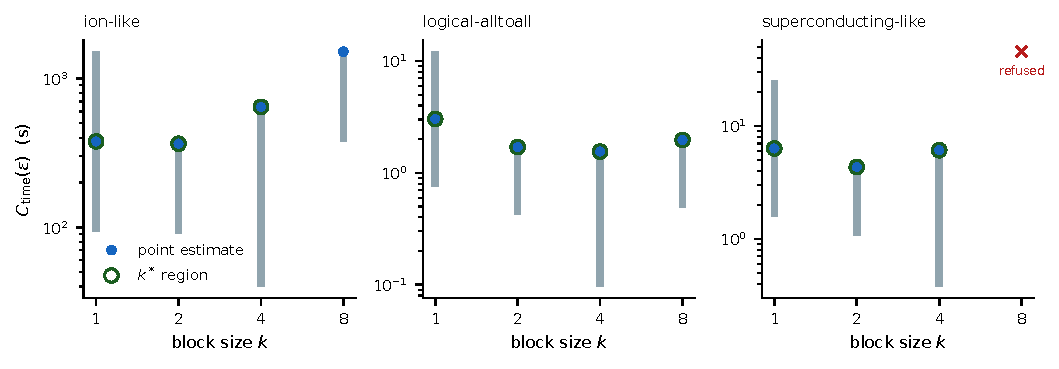
\includegraphics[width=\textwidth]{paper_assets/cost_bracket.pdf}
  \caption{Accuracy-matched cost brackets for the priced BeH$_2$ instance,
  Jordan--Wigner arm, single-assignment estimator.  Grey bars span the
  confirmed-failing to confirmed-passing interval; the open circle marks
  membership in the $k^*$ region.  Each panel has its own vertical scale: the
  three cards differ by orders of magnitude in gate time, which is the point of
  pricing under a card rather than counting settings.  A rung the card refuses
  carries no cost at all and is marked at the top of its panel.}
  \label{fig:cost}
\end{figure*}

Table~\ref{tab:cost} and Fig.~\ref{fig:cost} report the priced BeH$_2$ instance
along the Jordan--Wigner arm.  Three readings matter architecturally.  First,
the optimal rung moves with the card and the estimator: it is $k=\cqcKStarIon{}$
on the slow-gate card under single-assignment estimation and
$k=\cqcKStarLogical{}$ on the logical baseline.  Every cell resolves to a region
rather than a point --- the slow-gate cell to $k \in \{\cqcKStarIonRegion\}$ ---
and the record reports that status rather than collapsing it to an argmin.  Second, the mapping axis is not small: at the
qubit-wise rung the spread between the cheapest and dearest fermionic encoding
is \cqcMappingSpreadKOne{} on this one instance, and Table~\ref{tab:cost}
reports it again at each card's own $k^*$.  Third, the sparse-connectivity
card refuses the full-commutation rung here too, and a refused rung is absent
from the bracket rather than assigned an infinite cost.

The search itself is labelled.  The record declares its search uncertainty as
heuristic --- it is a Monte Carlo bracketing on a fixed shot grid, not a
certificate --- and separately declares the benchmark comparison as exact-tier
against an oracle reference.  Those two labels sit in the same file and are not
merged.  A cross-check against the independently produced shot-search record
agrees on \cqcCrossAgreeing{} of \cqcCrossChecked{} compared crossings, and the
record classifies each disagreement as environment-marginal rather than
substantive.

\section{What the architecture stopped}
\label{sec:stopped}

The results in this section are the reason the paper exists.  Each began as a
preregistered question with a declared gate, and each returned an answer that
stopped or narrowed the work rather than extending it.  In a framework without
an evidence contract, most of them would have been reported as something else
or not reported at all.

\subsection{A bank whose own bias exceeds the target is never priced}

The accuracy-matched search of the previous section covers two systems, and
only one of them is priced.  The H$_4$ bank carries an exact subspace bias of
\cqcHFourBias{}~mHa against a \cqcTargetMilliHartree{}~mHa target, so no shot
budget can bring its error inside the target: the deterministic part of the
error is already outside.  The record's status for that system is not a large
cost or a censored interval but \emph{bias floor exceeds target}, and no cost is
reported for it anywhere.  The priced BeH$_2$ bank of Sec.~\ref{sec:admitted}
clears the same floor with room to spare, at \cqcBeHBias{}~mHa, which is why it
has a price at all.

This is a small thing that is easy to get wrong.  The same pipeline, with the
bias and the statistical radius merged into one error bar, would have returned
a number --- a large one, but a number --- and that number would have entered a
cost comparison as though it were a price.  Separating the exact-tier bias from
the finite-sample radius at the type level is what turns it into a refusal.

\subsection{Mapping spread against instance spread: negative, then
indeterminate}

\begin{table*}
  \caption{Mapping spread against instance spread, on every tier that measured
  it.  The aggregation column is not decoration: the three readouts combine
  cells differently, and their numbers are not comparable across rows.}
  \label{tab:qr3}
  \footnotesize
  \begin{ruledtabular}
  \begin{tabular}{llp{0.20\textwidth}rrp{0.22\textwidth}}
  Readout & Tier & Aggregation & Mapping & Instance & Verdict \\
  \colrule
  % source-git-blob-sha: 196bfc37270c18d1376c437b1598e2df918cdda1
% source-git-blob-sha: 5f2faba83d1533d5a8ac4e40432cc294d9aff676
% source-git-blob-sha: 795860f11c1d6baa614683b0035013168a0b0c9b
% generator-git-blob-sha: 13f71027554c4af7ced72cd513c927ab28a040eb
QWC settings, matched greedy & structural & widest mapping vs.\ narrowest instance & \ensuremath{13.07} & \ensuremath{3.98} & mapping spread not smaller than instance spread \\
Mean Pauli word weight & structural & widest mapping vs.\ narrowest instance & \ensuremath{1.57} & \ensuremath{1.49} & mapping spread not smaller than instance spread \\
\colrule
Accuracy-matched $C_{\mathrm{time}}(\epsilon)$ & exact & point estimate on the supporting cells & \ensuremath{17.52} & \ensuremath{1.02} & indeterminate at this shot grid \\
Accuracy-matched $C_{\mathrm{time}}(\epsilon)$ & exact & conservative support of the same cells & \ensuremath{1.36} & \ensuremath{4.08} & indeterminate at this shot grid \\
R3d midpoint refinement & exact & support after added endpoints & \ensuremath{2.19} & \ensuremath{4.00} & indeterminate after refinement \\

  \end{tabular}
  \end{ruledtabular}
\end{table*}

A natural design question for a framework that supports several fermionic
encodings is whether the encoding choice matters more than the problem
instance.  If it does, an encoding-selection layer is worth building.  The
question was asked on three tiers and Table~\ref{tab:qr3} reports all of them.

Structurally, on matched greedy qubit-wise settings across the instances that
share one grouping protocol, the widest mapping spread within a system is
\cqcStructuralMapping{} while the narrowest instance spread across systems is
\cqcStructuralInstance{}; the declared margin is \cqcStructuralMargin{}, and the
verdict recorded is that mapping spread is not smaller than instance spread.
The same comparison on algorithm-independent word weight returns the same
verdict.  The structural readout is therefore negative in the direction that
would have justified the layer.

Accuracy-matched, a second instance was priced specifically to make the
comparison possible: \cqcRThreeCCells{} cells evaluated, \cqcRThreeCFinite{}
with a finite cost interval, \cqcRThreeCCensored{} right-censored at the grid
ceiling, over \cqcRThreeCSolves{} confirmatory solves with
\cqcRThreeCFailures{} failures, of which the sparse-connectivity card admits
only \cqcRThreeCSCPriced{}.  A censored cell is recorded as censored rather than
assigned an infinite cost or quietly dropped, and it licenses no wider grid.  On
that evidence the point estimates favour the mapping axis, but the conservative
supports of the same cells overlap, and the recorded verdict is
\emph{indeterminate at this shot grid}.  A targeted refinement then added
\cqcRThreeDCells{} within-grid endpoint cells chosen before any new draw, and the
supports still overlap: minimum possible mapping spread
\cqcRThreeDMappingSupport{} against maximum possible instance spread
\cqcRThreeDInstanceSupport{}, classified \emph{indeterminate after refinement}.

The refinement record also states its own asymmetry, which is the part we most
want to preserve here: because it targeted the parent record's point-support
cells rather than refining every cell entering the global extrema, a failure to
separate cannot establish the opposite direction.  It can only fail to
establish this one.  An architecture that allowed a non-separating outcome to be
written up as evidence for the converse would have produced a publishable claim
from this data.  This one produced \emph{indeterminate}, twice, and the
encoding-selection layer was not built.

\subsection{A screen that stopped before drawing a sample}

\begin{table*}
  \caption{The contextual-restriction admission screen on one BeH$_2$ bank.
  Rows are restriction rungs indexed by the number of fixed qubits.  Bias and
  word universe are given for the two contextually restricted arms; the two
  unrestricted arms are rung-independent and are stated in the last line.  The
  last column counts how many of the four arms are admissible, out of four.}
  \label{tab:r4a}
  \footnotesize
  \begin{ruledtabular}
  \begin{tabular}{rrrrrrrr}
  Fixed & Active & CS-QSE bias (mHa) & CS-QSE words & CS-A-CASE bias (mHa) & CS-A-CASE words & $H$ removed & Arms admitted \\
  \colrule
  % source-git-blob-sha: 7e480343cf4271073fa07da75c217d99625ac929
% generator-git-blob-sha: 7b19ec21a68f3d29a4b32ad8ae7b8c571b1d0fae
\ensuremath{1} & \ensuremath{7} & \ensuremath{5.35} & \ensuremath{3{,}864} & \ensuremath{5.90} & \ensuremath{40} & \ensuremath{15.3\%} & \ensuremath{1} \\
\ensuremath{2} & \ensuremath{6} & \ensuremath{5.35} & \ensuremath{997} & \ensuremath{5.90} & \ensuremath{33} & \ensuremath{15.3\%} & \ensuremath{1} \\
\ensuremath{3} & \ensuremath{5} & \ensuremath{5.90} & \ensuremath{124} & \ensuremath{5.90} & \ensuremath{19} & \ensuremath{15.4\%} & \ensuremath{1} \\
\ensuremath{4} & \ensuremath{4} & \ensuremath{5.90} & \ensuremath{14} & \ensuremath{5.90} & \ensuremath{14} & \ensuremath{15.4\%} & \ensuremath{1} \\
\ensuremath{5} & \ensuremath{3} & \ensuremath{5.90} & \ensuremath{6} & \ensuremath{5.90} & \ensuremath{6} & \ensuremath{15.5\%} & \ensuremath{1} \\
\ensuremath{6} & \ensuremath{2} & \ensuremath{5.90} & \ensuremath{3} & \ensuremath{5.90} & \ensuremath{3} & \ensuremath{15.5\%} & \ensuremath{1} \\
\ensuremath{7} & \ensuremath{1} & \ensuremath{5.90} & \ensuremath{1} & \ensuremath{5.90} & \ensuremath{1} & \ensuremath{15.5\%} & \ensuremath{1} \\
\colrule
\multicolumn{8}{p{0.96\textwidth}}{Unrestricted arms, identical at every rung: \texttt{full\_qse} bias \ensuremath{0.0033} mHa, word universe \ensuremath{14{,}350} (ceiling \ensuremath{2{,}048}); \texttt{acase} bias \ensuremath{0.0695} mHa, word universe \ensuremath{1{,}223}. Admissible bias \ensuremath{0.533} mHa.} \\

  \end{tabular}
  \end{ruledtabular}
\end{table*}

Contextual subspace methods restrict a Hamiltonian onto a stabilizer sector
chosen for the correlation it retains rather than for an exact symmetry
\cite{kirby2021contextual}, which makes them a natural preconditioner for an
operator-response subspace solver, and a dangerous one: the restriction is
approximate where symmetry tapering \cite{bravyi2017tapering} is exact.  The
screen in Table~\ref{tab:r4a} asks whether any restriction rung admits all four
comparison arms at once under gates fixed in advance --- an admissible bias
budget of \cqcRFourAAdmissibleBias{}~mHa, a word-universe ceiling of
\cqcRFourACeiling{}, and a fixed grouping rule.

None of the \cqcRFourARungs{} rungs admits all four arms; \cqcRFourAPassing{}
rungs pass.  The failure is structural and it comes from both ends.  The
unrestricted quantum-subspace-expansion reference arm overruns the
word-universe ceiling several times over, at \cqcRFourAFullWords{} words.  The
two contextually restricted arms come in far under the ceiling, some at a
handful of words, but they remove \cqcRFourARemovedFraction{} of the
Hamiltonian's non-identity Hilbert--Schmidt norm.  The CS-QSE arm carries a
bias of \cqcRFourACSBias{}~mHa and the CS-A-CASE arm carries
\cqcRFourACSACaseBias{}~mHa, both an order of magnitude past the admissible
budget.  The
unrestricted operator-response arm is the only one admissible at every rung, at
\cqcRFourAACaseBias{}~mHa over \cqcRFourAACaseWords{} words, and one admissible
arm does not make a rung: the screen compares four arms or it compares nothing.
There is no rung where the cheap arms are accurate enough and the accurate arm
is cheap enough.

The record's status is therefore \emph{structural screen complete, no samples},
its authorization field says that sampled execution was not authorized, and the
dependent phase that would have built the preconditioner is marked
not-authorized in the plan ledger.  The screen draws no samples at all: it is deterministic linear algebra over
the same restriction primitive the exact tapering path uses, and it stood in
for the sampling campaign that would otherwise have followed.  That is the
economic argument for this architecture, and it is the only one in this paper
that needs no device card.

\subsection{A reformulation that reproduced its predecessor}

A geometric-algebra structural preconditioner was proposed as a pre-encoding
filter chain, with two dependent phases scoped behind it.  The falsifier was
declared before the measurement: if the filters reproduce the existing
post-encoding filters and the action-equivalence quotient removes nothing, the
proposal is a reformulation and the dependent phases do not run.

The measured outcome is split by candidate pool, and the record says so rather
than choosing the flattering half.  The quotient removes \cqcGOneMajorana{}
candidates from the wide Majorana-monomial pool and \cqcGOneExcitation{} from
the determinant-excitation pool that every mapping and cost record is actually
built on.  At the matched degree cap the surviving Majorana classes reach
exactly the determinants the excitation pool reaches, so the chain reconstructs
that pool rather than producing a smaller one.  The verdict recorded is
``not falsified, but the content is pool-dependent'', the two dependent phases
were retired against it, and the record carries an explicit statement that
nothing in it licenses a resource claim of any kind.

\subsection{The ledger}

\begin{table*}
  \caption{The adjunct-programme ledger, read from the gated plan status file.
  Status and outcome are the file's own fields.}
  \label{tab:ledger}
  \footnotesize
  \begin{ruledtabular}
  \begin{tabular}{llll}
  Programme & Title & Status & Recorded outcome \\
  \colrule
  % source-git-blob-sha: 646a12f35feb98041cfe7c3c2776bb24370284ee
% generator-git-blob-sha: d4dfc704534ba3e9ea7f5cff4c04b8793b7bfde0
\texttt{A0-A5} & Paper A programme & complete & implemented and manuscript checked \\
\texttt{2M} & Memory-bounded matrix-element bank & partial & packed and stream recompute shipped small system equivalence tested full molecular matrix open \\
\texttt{4R} & Pooled reconstruction and rank selection & complete & implemented off by default \\
\texttt{PRD} & Preconditioned residual Davidson and WISE split & complete & exact positive finite shot negative \\
\texttt{G1} & GA structural preconditioner & complete & pool dependent content \\
\texttt{G2-G3} & GA mapping and cost decomposition & retired & g1 pools coincide at matched cap \\
\texttt{R1} & Hardware-aware cost infrastructure & complete & implemented and priced \\
\texttt{R2a-R2b} & Restriction primitive and mapping axis & complete & qr2 passes qr3 fixed qwc negative \\
\texttt{R3-R3d} & Protocol-cost and QR3 refinement programme & complete & second instance priced qr3 indeterminate \\
\texttt{R4a} & Contextual-subspace structural comparator & closed negative & no jointly admissible rung \\
\texttt{R4b} & CS-preconditioned A-CASE & not authorized & r4a did not authorize sampling or preconditioner build \\
\colrule
\multicolumn{4}{p{0.96\textwidth}}{Numbered phases: \ensuremath{15} of \ensuremath{20} complete (\ensuremath{75.0\%} strict, \ensuremath{81.2\%} progress-weighted); \ensuremath{5} open, partial, or proposed.} \\

  \end{tabular}
  \end{ruledtabular}
\end{table*}

Table~\ref{tab:ledger} is the plan status file, which is machine-readable and
gated in continuous integration against the plan document and the source tree.
Of \cqcNumberedPhases{} numbered phases, \cqcCompletePhases{} are complete:
\cqcStrictFraction{} strictly, or \cqcWeightedFraction{} weighted by partial
implementation.  Of the \cqcAdjunctPrograms{} adjunct programmes,
\cqcNegativePrograms{} ended in retirement, a closed-negative verdict, or a
phase that was never authorized, and one more is recorded as positive at the
exact tier and negative under finite shots.

We include this table because a research framework's plan is itself a claim,
and an ungated plan drifts toward describing the work that succeeded.  Gating
it means a phase cannot quietly change status between the commit that made it
and the paper that reports it.

\section{Scope and limitations}
\label{sec:limits}

We state the boundaries of this paper plainly, because a paper about
over-claiming has no excuse for any.

\paragraph{Instance scale.}  Every quantitative result here is on a small
active space, constructed from committed integral files
\cite{knowles1989fcidump,sun2018pyscf}.  All the priced and sampled banks are
eight-qubit; the widest instance entering any structural readout is a
twelve-qubit water active space, and it is excluded from the cross-instance
setting-count verdict for using a different cover heuristic.  Nothing in this
paper is a scaling result, and the block-size trade in particular is explicitly
instance-dependent in the only two instances measured.

\paragraph{Device cards are illustrative.}  Each card carries a calibration
status field, and the two non-baseline cards declare themselves illustrative
project scenarios rather than vendor data.  Routing is a declared scalar
surrogate, not a compiled layout.  Every runtime in this paper is logical
accounting, and none of it is a hardware measurement or a prediction about a
named device.

\paragraph{Search uncertainty is heuristic.}  The accuracy-matched costs come
from Monte Carlo bracketing on a fixed shot grid with declared replica counts.
The records label that uncertainty heuristic, separately from the exact-tier
label on the oracle comparison, and this paper does not merge them.

\paragraph{The negative results are bounded by their own scope.}  The
contextual screen is one bank under one set of declared gates; it does not
establish that contextual restriction cannot help an operator-response solver
in general, only that no rung of this screen admitted all four arms.  The
mapping-versus-instance refinement establishes nothing in the converse
direction, by its own recorded asymmetry.

\paragraph{The evidence contract has a gap.}
Section~\ref{sec:evidence} quantifies it: a record can be committed today
without a top-level evidence tier, and \cqcRecordsUnlabelled{} of them are.  The
census makes that visible on every rebuild; it does not prevent it.

\paragraph{Not a comparison against other frameworks.}  \pkg{} bridges to the
external ecosystem rather than competing with it, and no benchmark in this
paper measures another package.  The architectural claim is about what this
design makes difficult to over-claim, not about relative capability or speed.

\section{Reproducibility}
\label{sec:reproducibility}

Every number in this manuscript, in the body text as well as in the tables, is
generated from a committed record or from a live census of the source tree.
The prose quantities are macros written by the table generator, and the
manuscript checker rejects any numeral typed into the body outside a short
allowlist of conceptual notation --- a block size under discussion, a chemical
subscript, the dimension of the algebra.  The generated fragments are checked
by regenerating them during the check and comparing byte for byte, which is
stronger than the content hashes they also carry: a hash over the inputs
catches a record regenerated without rerunning the generator, but only
regeneration catches a value edited into a fragment by hand.  Figures are bound the same way through a manifest
of input digests, because vector output is not byte-reproducible across plotting
and font builds while the digest of its inputs is.

Two checks exist specifically to keep this paper honest about the architecture
it describes.  The layer census fails if any module of the package is not
assigned to exactly one layer, and the gate census fails if any benchmark gate
has no declared class.  Both would otherwise be the first tables to drift, being
the ones no experiment rebuilds.

\section{Discussion}
\label{sec:discussion}

The results in Sec.~\ref{sec:stopped} have a common shape.  In each, a
quantity that looks like a number --- a cost, a spread, a reduction --- turned
out to be a number only under conditions that a less strict architecture would
not have made explicit: a bias floor that must be cleared before a price
exists; a fidelity floor that makes a protocol unpriceable rather than
expensive; supports that overlap even when point estimates separate; a
restriction that buys width by removing Hamiltonian norm.  None of these are
deep results.  All of them are the kind of thing that becomes a published claim
when the pipeline that produces it has no place to record the qualification.

We would draw three transferable conclusions.  First, admissibility belongs in
the cost type.  A cost model that can only return numbers will return one for a
protocol the device cannot run.  Second, preregistration is cheap in software.
A configuration file with a content hash and a merge commit, landed before
sampling, costs one pull request and converts a null result from an
embarrassment into an artifact.  Third, a census beats a description.  The
tables in Secs.~\ref{sec:architecture} and \ref{sec:gates} are recomputed on
every build, and the one that most needed that treatment was the unflattering
one in Sec.~\ref{sec:evidence}, which we would not have quantified at all if the
architecture had not been asked to measure itself.

\paragraph{Streamlining options.}
The same diagram suggests three smaller operational profiles, none of which is
a result of the present benchmarks.  The lowest-risk simplification is a
five-contract spine --- model, restriction, solver, estimator and evidence
record --- with the existing implementations selected as policies behind those
interfaces.  This preserves every comparator while removing orchestration from
the scientific contracts.  A method-centred profile would make A-CASE the only
production solver, retain QSCI and selected CI as validation controls, and use
ADAPT-VQE only as an optional warm start; that yields the clearest method story
but narrows the production surface.  An execution-centred profile would split
offline bank construction and measurement-plan compilation from online
sampling and cumulative-cache updates; it reduces repeated work without
changing the solver family.  The interface spine is the natural first move,
because it also gives exact and measured response one estimator path instead
of parallel implementations.  These are design alternatives, not performance
claims.

The obvious next step is the gap this paper names: a required evidence tier,
schema-validated over every committed record, so that the contract enforced in
code is also enforced at the boundary where records are written.  That is a
smaller change than any of the phases in Table~\ref{tab:ledger}, and on the
evidence of Table~\ref{tab:evidence} it is the most valuable one available.

\section{Conclusion}
\label{sec:conclusion}

We have described \pkg{} as an architecture rather than as a capability list:
one sparse Pauli-word algebra shared by a numerical kernel and an explicit
program-IR container, evidence labels carried from the measurement layer into
committed records where declared, and a
benchmark layer of paired producers and gates with preregistration where a
result could otherwise be chosen after the fact.  The evidence we offer for the
architecture is the evidence it produced, including a certified shot reduction
that one device card refuses to price, an accuracy-matched optimum that belongs
to the card rather than the Hamiltonian, a bank that is never priced because its
own bias exceeds the target, two preregistered screens that returned no result,
a reformulation retired against its own falsifier, and a coverage census that
shows where the contract is not yet enforced.  Not one of these is an advantage
claim, and that is the point: the architecture's value is measured by what it
would not let us say.

\begin{acknowledgments}
We thank the maintainers of the open-source quantum software ecosystem that
\pkg{} bridges to.  The framework is a pre-release research codebase; the
records, generators, gates and tests that produced every number in this
manuscript are versioned together.
\end{acknowledgments}

\bibliographystyle{apsrev4-2}
\bibliography{references}

\end{document}
